\documentclass{article}
\usepackage{main}

\title{Phishing}
\author{}
\date{2 Février 2024}

\begin{document}
\maketitle

Lire \url{https://www.economie.gouv.fr/particuliers/phishing-hameconnage-filoutage#} (chercher \url{phishing economie.gouv} sur google) et répondre aux questions suivantes :
\begin{enumerate}
\item Qu'est-ce que le phishing (ou hammeçonage en français) ?
\item Donner des exemples possibles de demandes formulées par un arnaqueur lors d'un fishing.
\item Quelles techniques parmi celles proposées par le site vous semblent les plus efficaces ? Avez-vous idée d'autres techniques ?
\item Dire si les mails suivants sont des tentatives de phishing, et préciser pourquoi.
\end{enumerate}

\begin{center}
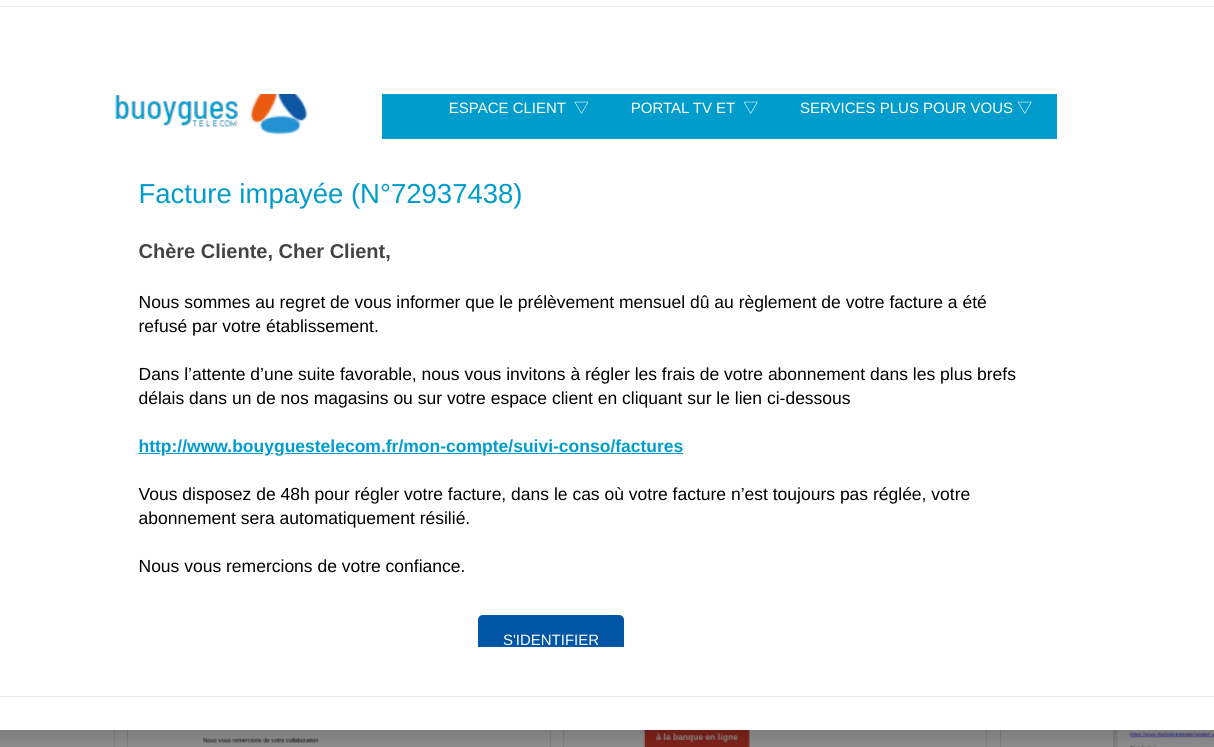
\includegraphics[scale=0.3]{buoygues.png}
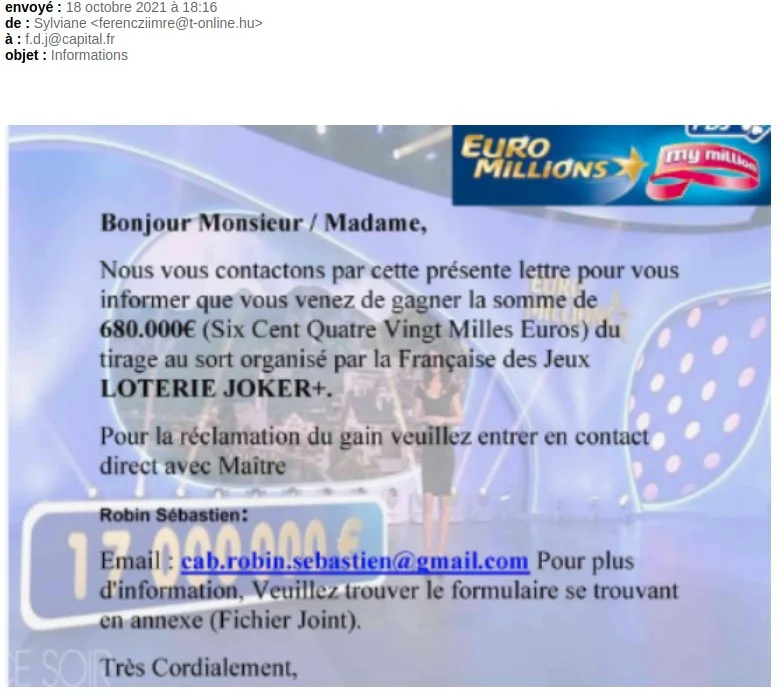
\includegraphics[scale=0.3]{loto.png}
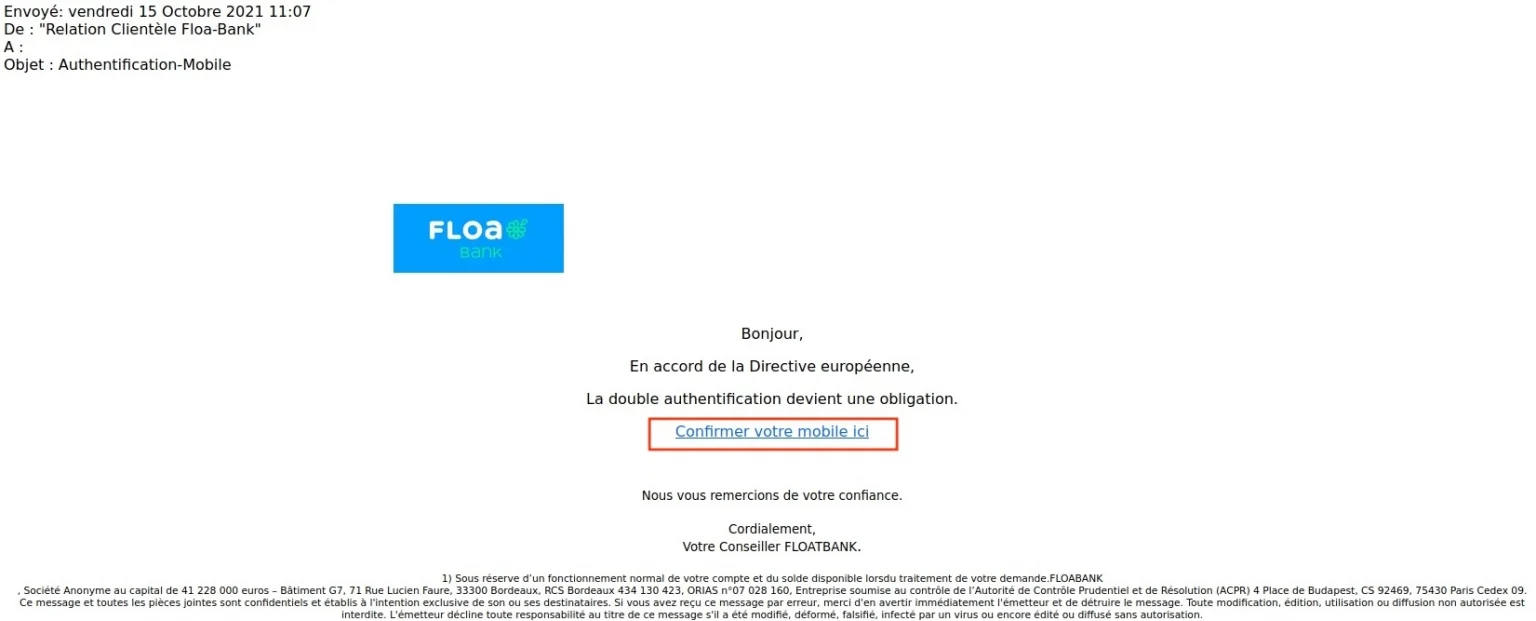
\includegraphics[scale=0.3]{float.png}
\end{center}
\end{document}